\documentclass[conference]{IEEEtran}
\IEEEoverridecommandlockouts
% Built against the Overleaf "IEEE Conference Template" (IEEEtran, conference option).
\usepackage{cite}
\usepackage{amsmath,amssymb,amsfonts}
\usepackage{graphicx}
\usepackage{textcomp}
\usepackage{xcolor}
\usepackage{booktabs}
\usepackage{multirow}
\usepackage{siunitx}
\usepackage{tikz}
\usetikzlibrary{positioning,arrows.meta,fit,calc}
\usepackage{pgfplots}
\pgfplotsset{compat=1.17}
\sisetup{detect-weight=true,group-minimum-digits=4}
\def\BibTeX{{\rm B\kern-.05em{\sc i\kern-.025em b}\kern-.08em
    T\kern-.1667em\lower.7ex\hbox{E}\kern-.125emX}}

\begin{document}

\title{VisionFood QAI: Distilled Bottle-Cap Defect Segmentation with Threshold Analysis and Geometric Fill-Level Estimation, Deployed with TensorRT}

\author{\IEEEauthorblockN{Ullas N, Nayana N Kumar, Sushanth S, and Shreyas Bairy K S}
\IEEEauthorblockA{\textit{Department of Computer Science and Engineering (Data Science)}\\
\textit{B.M.S. College of Engineering (Autonomous Institute, Affiliated to VTU)}\\
Bengaluru 560019, India\\
Corresponding author: ullasn.cd23@bmsce.ac.in}}

\maketitle

\begin{abstract}
We present and evaluate the two inspection stations of VisionFood QAI, a vision system for transparent beverage bottles. Station~1 inspects the closure with a YOLO11m instance-segmentation student (22.3\,M parameters). It is distilled from a YOLO11x-seg teacher (62.1\,M) through feature alignment at the C3k2, SPPF, and C2PSA modules, and labels six cap states (good, damaged, misplaced, missing, open, wet) on three synchronised camera views. An asymmetric quality gate turns its detections into PASS, REJECT, UNCERTAIN, or INSPECTION\_FAILED. Station~2 estimates fill level from a bottle detector, a liquid-surface (meniscus) detector, and a closed-form fill ratio with configurable underfill/overfill thresholds. On the held-out test split of the public six-class cap dataset, the student matches the teacher's mAP@0.5 of 0.995 with 2.8$\times$ fewer parameters, and exceeds the teacher's mask mAP@0.5:0.95 (0.927 vs.\ 0.912). As a deployed FP16 TensorRT engine it reaches mask mAP@0.5:0.95 of 0.928. Replaying the production gate gives zero false accepts (0/153 defective caps) and zero false rejects (0/201 good caps). A threshold sweep shows that good-cap scores lie in $[0.856, 0.921]$, which leaves a 0.106 margin above the default pass bar of 0.75. For fill level, the meniscus detector reaches AP@0.5 of 0.923 on its test split. The median fill-ratio error caused by meniscus localisation is 0.002, and 34 of 35 verdicts agree with those computed from the annotated surface. TensorRT FP16 cuts the three-view network time from 21.0\,ms (PyTorch FP32) to 7.4\,ms. In a Docker stress test the complete closed loop, including synchronous audit storage of 2048-pixel frames, runs at a median of 299\,ms per bottle, and the fill station at 62.8\,ms.
\end{abstract}

\begin{IEEEkeywords}
bottle-cap inspection, instance segmentation, YOLO11, knowledge distillation, fill-level estimation, TensorRT, threshold analysis, quality gate
\end{IEEEkeywords}

%=====================================================================
\section{Introduction}
Closure and fill-level defects are the two most frequent visual rejects on beverage bottling lines. A missing, open, or misplaced cap compromises the seal, and an underfilled or overfilled container violates declared-volume requirements. Manual inspection does not scale to line rates of several bottles per second~\cite{banus2021}. Learned detectors are attractive, but published food-packaging inspectors often report only validation-set accuracy, without product-level error rates or deployment latency~\cite{liu2025,chatchapol2024}.

This paper reports the final iteration of a capstone system and narrows its scope to what we have built and measured. It covers two stations for transparent PET bottles. Station~1 inspects caps and Station~2 measures fill level. Product types other than transparent bottles, label checks, and operator-interface features are out of scope and are not claimed. The contributions follow the project objectives:
\begin{itemize}
\item \textbf{Distilled cap segmentation with threshold analysis.} We distil a YOLO11x-seg teacher into a YOLO11m-seg student through L2-normalised feature alignment at three YOLO11 modules, and pair it with an asymmetric multi-view gate. We evaluate the FP32 and deployed FP16 student on the held-out split with per-class, image-level, and product-level (false-accept/false-reject) metrics, and we map how the gate's thresholds trade review load against error.
\item \textbf{Dataset and artefact characterisation (O1).} We document the six-class dataset (per-split, per-class counts, capture resolution, object-size distribution) and the exported artefacts (PyTorch, ONNX, TensorRT), and we verify that the FP16 engine preserves the student's accuracy.
\item \textbf{Geometric fill-level estimation (O2).} We formalise the deployed bottle/meniscus association and the trimmed fill-ratio rule, derive its sensitivity to localisation error, and measure the fill-ratio error and verdict agreement caused by meniscus localisation on held-out images.
\item \textbf{Deployment optimisation (O3).} We export all three models to TensorRT FP16 engines, measure per-stage latency against PyTorch and ONNX Runtime baselines, and stress-test the complete pipeline in its Docker deployment.
\end{itemize}

%=====================================================================
\section{Related Work}
\textit{Food and beverage inspection.} Liakos \textit{et al.}~\cite{liakos2025} survey machine learning for food quality control and report that beverages are a small minority of the studied applications. Chatchapol \textit{et al.}~\cite{chatchapol2024} classify beverage fill levels with a CNN on an embedded GPU but do not localise the liquid surface. Farhangi \textit{et al.}~\cite{farhangi2024} inspect liquid bottles with rule-based edge detection and pattern matching. Liu \textit{et al.}~\cite{liu2025} detect five packaging defects with an attention-augmented YOLOv5. Banús \textit{et al.}~\cite{banus2021} compare CNN backbones for thermoformed food packages. None of these works reports product-level false-accept and false-reject rates or end-to-end deployment latency.

\textit{Real-time segmentation.} Ultralytics YOLO11~\cite{yolo11} and YOLOv8~\cite{yolov8} are anchor-free one-stage detectors. Their segmentation variants predict per-instance coefficients over a set of mask prototypes, following YOLACT~\cite{bolya2019}.

\textit{Knowledge distillation.} Response distillation transfers softened logits~\cite{hinton2015}. Hint-based distillation aligns intermediate features through learned projectors~\cite{romero2015}. Feature imitation has been applied to object detectors to compress them for deployment~\cite{wang2019}.

%=====================================================================
\section{System Overview}
Fig.~\ref{fig:pipeline} shows both stations. Station~1 receives three synchronised views of each bottle (front, rear, side). The three views pass through the network as one batch, and non-maximum suppression (NMS) is applied separately to each image. Each view is judged independently, and the bottle verdict is \emph{defect-dominant}: a defect seen by any camera rejects the bottle. Station~2 receives one side view and runs two single-image detectors followed by a geometric rule. Both stations run the same export chain (Section~\ref{sec:deploy}).

\begin{figure}[t]
\centering
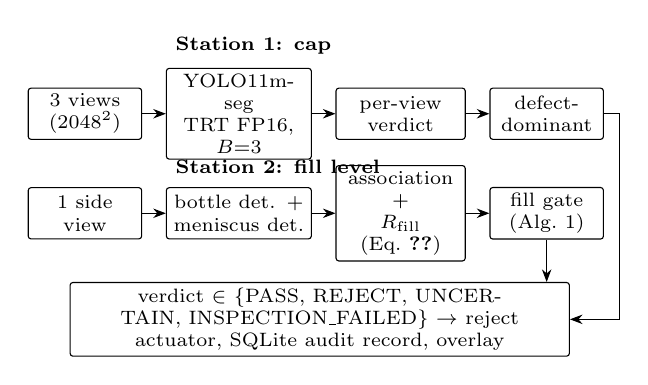
\begin{tikzpicture}[node distance=2.2mm and 3mm, font=\scriptsize,
  box/.style={draw, rounded corners=1pt, align=center, minimum height=6.5mm, inner sep=2pt, text width=#1},
  box/.default=17mm, >={Stealth[length=1.6mm]}]
\node[box=13mm] (cams) {3 views\\(2048$^2$)};
\node[box=17mm, right=of cams] (seg) {YOLO11m-seg\\TRT FP16, $B{=}3$};
\node[box=15mm, right=of seg] (view) {per-view\\verdict};
\node[box=13mm, right=of view] (agg) {defect-\\dominant};
\draw[->] (cams) -- (seg); \draw[->] (seg) -- (view); \draw[->] (view) -- (agg);
\node[font=\scriptsize\bfseries, above=0.5mm of seg.north west, anchor=south west] {Station 1: cap};
\node[box=13mm, below=6mm of cams] (cam2) {1 side\\view};
\node[box=17mm, right=of cam2] (det) {bottle det. +\\meniscus det.};
\node[box=15mm, right=of det] (ratio) {association +\\$R_{\mathrm{fill}}$ (Eq.~\ref{eq:ratio})};
\node[box=13mm, right=of ratio] (fgate) {fill gate\\(Alg.~1)};
\draw[->] (cam2) -- (det); \draw[->] (det) -- (ratio); \draw[->] (ratio) -- (fgate);
\node[font=\scriptsize\bfseries, above=0.5mm of det.north west, anchor=south west] {Station 2: fill level};
\coordinate (mid) at ($(det.south)!0.5!(ratio.south)$);
\node[box=62mm, below=4mm of mid] (out) {verdict $\in$ \{PASS, REJECT, UNCERTAIN, INSPECTION\_FAILED\} $\rightarrow$ reject actuator, SQLite audit record, overlay};
\draw[->] (agg.east) -- ++(2mm,0) |- (out.east);
\draw[->] (fgate.south) -- (fgate.south |- out.north);
\end{tikzpicture}
\caption{The two inspection stations evaluated in this paper. Both use TensorRT FP16 engines compiled on the target GPU.}
\label{fig:pipeline}
\end{figure}

%=====================================================================
\section{Station 1: Cap Inspection}
\subsection{Dataset}
We use the public \texttt{bottle\_cap\_sdp} v7 dataset~\cite{capdata} (CC BY 4.0). It contains polygon instance masks for six classes. Table~\ref{tab:capdata} gives the counts we found on disk. The Roboflow export notes 8{,}530 images, but the three splits contain 8{,}524. Every image shows one bottle neck with one annotated cap, captured at $2048{\times}2048$ (a handful at $2048{\times}1536$) against indoor backgrounds. The training split holds 2{,}486 source photographs, each exported in three augmented versions (rotation $\pm5^\circ$, brightness $\pm25\%$, Gaussian blur up to 2\,px, 0.5\% salt-and-pepper noise). Validation and test images are unaugmented. The masks come from a single annotator, so inter-annotator agreement cannot be measured.

\begin{table}[t]
\caption{Six-class cap dataset (instances = images; one cap per image)}
\label{tab:capdata}
\centering
\begin{tabular}{lrrr}
\toprule
Class & Train & Valid & Test\\
\midrule
good\_cap & 4{,}242 & 405 & 201\\
wet\_cap & 828 & 79 & 39\\
open\_cap & 768 & 65 & 38\\
damaged\_cap & 648 & 62 & 31\\
no\_cap & 645 & 61 & 30\\
misplaced\_cap & 327 & 40 & 15\\
\midrule
Total images & 7{,}458 & 712 & 354\\
Source photographs & 2{,}486 & 712 & 354\\
\bottomrule
\end{tabular}
\end{table}

The cap is not a small object in this dataset. Its median bounding box covers 9.2\% of the test image (10th--90th percentile: 6.0--14.0\%). After resizing to the $640{\times}640$ network input, every instance is ``large'' by the COCO definition ($\geq96^2$\,px)~\cite{coco}. The fine-scale content lies \emph{inside} the cap: droplets on wet caps, dents on damaged caps, and the thread gap of open caps. For this reason we analyse accuracy by object size in Section~\ref{sec:capresults} but do not claim small-object detection.

\subsection{Model and Training}
The deployed model is the distilled YOLO11m-seg student~\cite{yolo11} (Section~\ref{sec:kd}), with 22.34\,M parameters and 113.0\,GFLOPs at 640\,px after layer fusion. It was initialised from COCO weights and trained at 640\,px with batch 32, using AdamW (initial learning rate $10^{-3}$, cosine decay to $10^{-5}$, 5 warm-up epochs, weight decay $5{\times}10^{-4}$). Loss gains were box 7.5, DFL 1.5, and classification 4.0. The classification gain is the mean majority-to-class count ratio (6.29), capped at 4.0. It is a single scalar and does not re-weight classes individually. Augmentation used mosaic (disabled for the last 10 epochs), copy-paste 0.5, mixup 0.15, rotation $\pm15^\circ$, translation 0.1, scale 0.5, vertical flip 0.3, horizontal flip 0.5, HSV jitter (0.015/0.7/0.4), RandAugment, and random erasing 0.4, with mixed precision and seed 42. Training stopped early at epoch 126 (patience 30, best epoch 96) after 5.3\,h on an NVIDIA RTX A5000 (Fig.~\ref{fig:curve}).

\begin{figure}[t]
\centering
\begin{tikzpicture}
\begin{axis}[width=\columnwidth, height=38mm, xlabel={epoch}, ylabel={val. mAP@0.5:0.95}, ymin=0.5, ymax=1.0, xmin=0, xmax=127,
  legend pos=south east, legend style={font=\scriptsize}, tick label style={font=\scriptsize}, label style={font=\scriptsize}, grid=major, grid style={gray!20}]
\addplot[blue, thick] table[x=epoch, y=maskmap] {figures/student_curve.dat};
\addplot[red, dashed] table[x=epoch, y=boxmap] {figures/student_curve.dat};
\draw[gray] (axis cs:96,0.5) -- (axis cs:96,1.0) node[pos=0.12, left, font=\scriptsize] {best (96)};
\legend{mask, box}
\end{axis}
\end{tikzpicture}
\caption{Validation mAP@0.5:0.95 of the YOLO11m-seg student during distillation training.}
\label{fig:curve}
\end{figure}

\subsection{Teacher--Student Feature Distillation}
\label{sec:kd}
The teacher is YOLO11x-seg~\cite{yolo11} (62.06\,M parameters, 297.4\,GFLOPs). It was trained on the same data with the student's optimiser, loss gains, and augmentation (Section~IV-B) at batch 16 for the full 150 epochs (12.2\,h; best epoch 139), and then frozen. Minute cap defects such as droplets, dents, and a thread gap occupy a small fraction of the cap region. Matching only the teacher's final outputs would tell the student \emph{what} to predict but not \emph{where} to look. We therefore distil intermediate features at three junctures of the YOLO11 architecture:
\begin{itemize}
\item \textbf{C3k2} (backbone output): edge and texture features, including thread and ridge geometry.
\item \textbf{SPPF} (backbone--neck transition): multi-scale pooled context, so that fine cues survive spatial down-sampling.
\item \textbf{C2PSA} (spatial attention): the teacher's attention map, which transfers where fine defect evidence lies.
\end{itemize}
Forward hooks capture these outputs in both networks. Learned $1{\times}1$ projectors $\phi_\ell$ lift student channels to teacher width (256$\to$512 and 512$\to$1024), following the hint-layer approach~\cite{romero2015}. The objective is
\begin{equation}
\mathcal{L}=\mathcal{L}_{\mathrm{YOLO}}+\alpha(t)\sum_{\ell}\bigl\lVert \hat F^{T}_{\ell}-\widehat{\phi_\ell(F^{S}_{\ell})}\bigr\rVert_2^2,
\end{equation}
where $\hat{\cdot}$ denotes channel-wise $L_2$ normalisation and $\alpha$ ramps linearly from 0.05 to 0.5 over 20 epochs. Normalisation keeps the large, uniform background from dominating the loss, so the student matches the \emph{pattern} of teacher activations rather than their magnitude. The ramp lets the student learn basic detection before the alignment pressure takes full effect. Teacher features are detached, so no gradient flows into the teacher. The projectors exist only during training and are discarded before export, so distillation adds no inference cost.

\textit{Outcome.} Table~\ref{tab:kd} compares teacher and student, both evaluated in FP32 with the same Ultralytics validation on the same splits. The student matches the teacher's mAP@0.5 of 0.995 on every class with 2.8$\times$ fewer parameters, 2.6$\times$ fewer FLOPs, and a 2.8$\times$ smaller checkpoint. Its per-image inference is 7.8\,ms, against 19.0\,ms for the teacher. At strict IoU the two models trade places. The student's \emph{mask} mAP@0.5:0.95 is higher than the teacher's (test 0.927 vs.\ 0.912; validation 0.936 vs.\ 0.913), and it is higher for five of the six classes; damaged caps are level (0.927 vs.\ 0.929). The gain is largest on the classes whose evidence is finest: wet (0.953 vs.\ 0.924), misplaced (0.941 vs.\ 0.899), and good (0.893 vs.\ 0.877). The teacher keeps a small lead in \emph{box} mAP@0.5:0.95 (0.944 vs.\ 0.927). Station~1 decides from the cap's mask, so this is the trade the application favours. The student also has higher test recall (1.000 vs.\ 0.997; the teacher misses one open cap) and produces no spurious background detection, where the teacher produces one.

\begin{table}[t]
\caption{Teacher vs.\ distilled student (FP32, 640\,px)}
\label{tab:kd}
\centering
\setlength{\tabcolsep}{3pt}
\resizebox{\columnwidth}{!}{%
\begin{tabular}{lcc}
\toprule
& Teacher & Student\\
& YOLO11x-seg & YOLO11m-seg\\
\midrule
Parameters (M) & 62.06 & 22.34\\
GFLOPs @640 & 297.4 & 113.0\\
Checkpoint size (MB) & 124.8 & 45.2\\
Inference per image (ms)$^\ast$ & 19.0 & 7.8\\
\midrule
\multicolumn{3}{l}{\textit{Test split ($n{=}354$)}}\\
Box P / R & 0.995 / 0.997 & 0.998 / 1.000\\
Box / mask mAP@0.5 & 0.995 / 0.995 & 0.995 / 0.995\\
Box mAP@0.5:0.95 & \textbf{0.944} & 0.927\\
Mask mAP@0.5:0.95 & 0.912 & \textbf{0.927}\\
\midrule
\multicolumn{3}{l}{\textit{Per-class mask mAP@0.5:0.95 (test)}}\\
damaged / good & 0.929 / 0.877 & 0.927 / \textbf{0.893}\\
misplaced / no\_cap & 0.899 / 0.913 & \textbf{0.941} / 0.915\\
open / wet & 0.931 / 0.924 & 0.935 / \textbf{0.953}\\
\midrule
\multicolumn{3}{l}{\textit{Validation split ($n{=}712$)}}\\
Box / mask mAP@0.5:0.95 & 0.946 / 0.913 & 0.938 / 0.936\\
\bottomrule
\multicolumn{3}{l}{\footnotesize $^\ast$PyTorch FP32 batch 1, Ultralytics val; teacher on its training GPU.}
\end{tabular}
}
\end{table}

\subsection{Why a Segmentation Detector}
Before choosing the architecture we benchmarked five whole-image cap classifiers on a separate four-class dataset (7{,}540 images; 308-image test split; image-level split). Table~\ref{tab:cls} summarises the results. The numbers come from a different dataset and label set, so they are not comparable with Station~1 results. They informed the design in two ways. First, even the best classifier fell below 0.86 F1 on the damaged-cap class. Second, a classifier gives no location, whereas the gate and the audit record need the cap's region (mask area, polygon, and per-view evidence). YOLO11m-seg provides class, box, and mask in one pass. Its three-view batch costs 7.4\,ms on the deployment GPU (Section~\ref{sec:deploy}).

\begin{table}[t]
\caption{Preliminary whole-image cap classifiers (separate 4-class dataset, $N_{\mathrm{test}}{=}308$). GPU: PyTorch, batch 1; CPU: ONNX Runtime INT8.}
\label{tab:cls}
\centering
\setlength{\tabcolsep}{3pt}
\resizebox{\columnwidth}{!}{%
\begin{tabular}{lrrrrrr}
\toprule
Model & Acc.\,\% & mF1\,\% & Dmg F1 & Par.\,M & GPU ms & CPU ms\\
\midrule
MobileNetV3-L~\cite{howard2019} & 96.43 & 94.75 & 0.857 & 4.21 & 9.36 & 4.77\\
EfficientNetV2-S~\cite{tan2021} & 95.78 & 93.96 & 0.831 & 20.18 & 38.86 & 20.82\\
ShuffleNetV2~\cite{ma2018} & 94.81 & 92.84 & 0.794 & 1.26 & 8.55 & 3.48\\
ResNet-50~\cite{he2016} & 94.81 & 92.30 & 0.788 & 23.52 & 13.14 & 11.19\\
DeiT-Tiny~\cite{touvron2021} & 94.81 & 92.69 & 0.788 & 5.53 & 12.64 & 7.07\\
\bottomrule
\end{tabular}
}
\end{table}

\subsection{Asymmetric Multi-View Quality Gate}
\label{sec:gate}
The network runs with a confidence floor of 0.35. For each view, the gate evaluates the rules in order:
(i) no detection $\Rightarrow$ INSPECTION\_FAILED;
(ii) any defect-class detection with score $\geq\tau_d{=}0.45$ $\Rightarrow$ REJECT;
(iii) top detection is good\_cap with score $\geq\tau_p{=}0.75$ $\Rightarrow$ PASS;
(iv) top detection is good\_cap with score in $[\tau_u, \tau_p)$, $\tau_u{=}0.40$ $\Rightarrow$ UNCERTAIN;
(v) otherwise UNCERTAIN.
The bottle verdict is REJECT if any view rejects, else INSPECTION\_FAILED if any view failed, else UNCERTAIN if any view is uncertain, else PASS. REJECT and INSPECTION\_FAILED fire the actuator. UNCERTAIN goes to human review without ejection. The thresholds are asymmetric by design: a lower bar to reject than to pass, so a doubtful cap is never auto-passed.

%=====================================================================
\section{Station 2: Fill-Level Estimation}
\subsection{Models and Data}
The \textit{bottle detector} is YOLOv8s~\cite{yolov8} (9.84\,M parameters, classes bottle and cap). It was trained at 512\,px for up to 150 epochs (AdamW, learning rate $10^{-3}$, batch 8, mosaic 0.8, mixup 0.15) on a merged collection of four public bottle and cap sources: 2{,}286/417/280 images in train/valid/test, with 2{,}133/774/356 bottle instances. The \textit{meniscus detector} is YOLOv8n (2.69\,M parameters, single class \texttt{water\_surface}). It was trained at 640\,px for 110 epochs without mosaic or mixup on a merge of two public sets~\cite{filldata1,filldata2}: 545/31/41 images and 1{,}683/54/76 surface boxes. One source set consists of frames from a video of a multi-bottle rack.

\subsection{Association and Fill Ratio}
For a frame of width $W$, the bottle detector runs at confidence $\geq0.25$, and the highest-scoring \emph{bottle} box $b=(x_1^b,y_1^b,x_2^b,y_2^b)$ is kept. The meniscus detector then runs on the full frame at confidence $\geq0.15$. A candidate surface box $w$ is associated with the bottle when its horizontal centre lies inside $[x_1^b,x_2^b]$ and either its top or its bottom edge lies inside $[y_1^b,y_2^b]$. Among associated candidates, the highest-scoring one is kept. With bottle height $h=y_2^b-y_1^b$, the bottle box is trimmed to compensate for detector padding:
\begin{equation}
y_1' = y_1^b+\lfloor0.03h\rfloor,\quad y_2' = y_2^b-\lfloor0.02h\rfloor,\quad h'=y_2'-y_1'.
\end{equation}
The surface height is the box mid-line, clamped to the trimmed bottle, $y_w=\min\bigl(y_2',\max(y_1',\lfloor (y_1^w+y_2^w)/2\rfloor)\bigr)$. The fill ratio is
\begin{equation}
R_{\mathrm{fill}}=\frac{y_2'-y_w}{h'}\in[0,1].
\label{eq:ratio}
\end{equation}
Fig.~\ref{fig:geom} illustrates the geometry. The thresholds $\theta_u{=}0.40$ and $\theta_o{=}0.85$ come from a single configuration source (environment variables). The gate, the overlay ruler, and the health endpoint all read the same values.

\begin{figure}[t]
\centering
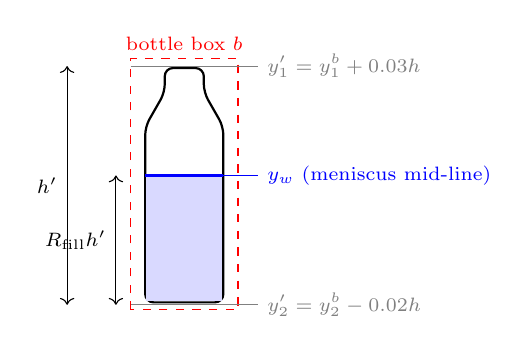
\begin{tikzpicture}[scale=0.62, font=\scriptsize]
\draw[thick, rounded corners=3pt] (0,0) -- (0,3.6) -- (0.4,4.3) -- (0.4,4.8) -- (1.2,4.8) -- (1.2,4.3) -- (1.6,3.6) -- (1.6,0) -- cycle;
\fill[blue!15] (0.02,0.02) rectangle (1.58,2.6);
\draw[blue, thick] (0,2.6) -- (1.6,2.6);
\draw[red, dashed] (-0.3,-0.15) rectangle (1.9,5.0);
\draw[gray] (-0.3,4.84) -- (2.3,4.84) node[right] {$y_1'=y_1^b+0.03h$};
\draw[gray] (-0.3,-0.05) -- (2.3,-0.05) node[right] {$y_2'=y_2^b-0.02h$};
\draw[blue] (1.6,2.6) -- (2.3,2.6) node[right] {$y_w$ (meniscus mid-line)};
\draw[<->] (-0.6,-0.05) -- node[left] {$R_{\mathrm{fill}}h'$} (-0.6,2.6);
\draw[<->] (-1.6,-0.05) -- node[left] {$h'$} (-1.6,4.84);
\node[red] at (0.8,5.3) {bottle box $b$};
\end{tikzpicture}
\caption{Fill-ratio geometry: trimmed bottle box (gray) and meniscus mid-line (blue). Image $y$ grows downwards.}
\label{fig:geom}
\end{figure}

\subsection{Fill Gate}
Algorithm~1 gives the decision rule. A borderline ratio (within $\pm\beta{=}0.02$ of either threshold) combined with low meniscus confidence (below $c_{\min}{=}0.50$) is sent to review instead of being auto-rejected. A missing bottle is treated as a conveyor gap and does not fire the actuator.

\begin{figure}[t]
\centering
\fbox{\begin{minipage}{0.94\columnwidth}\small
\textbf{Algorithm 1} (fill gate)\\[2pt]
\textbf{if} no bottle \textbf{then} INSPECTION\_FAILED (no actuation)\\
\textbf{else if} no associated meniscus \textbf{then} REJECT (empty/opaque)\\
\textbf{else if} $\min_{\theta\in\{\theta_u,\theta_o\}}|R-\theta|\le\beta$ \textbf{and} $c_w<c_{\min}$ \textbf{then} UNCERTAIN\\
\textbf{else if} $R<\theta_u$ \textbf{then} REJECT (underfill)\\
\textbf{else if} $R>\theta_o$ \textbf{then} REJECT (overfill)\\
\textbf{else} PASS
\end{minipage}}
\end{figure}

\subsection{Sensitivity of the Rule}
\label{sec:sens}
Differentiating Eq.~\eqref{eq:ratio} gives
\begin{equation}
\frac{\partial R}{\partial y_w}=-\frac{1}{h'},\qquad \frac{\partial R}{\partial y_1'}=\frac{R}{h'},\qquad \frac{\partial R}{\partial y_2'}=\frac{1-R}{h'}.
\end{equation}
An error of $\delta$ pixels in the meniscus therefore shifts $R$ by $\delta/h'$. For the median bottle in our test images ($h{=}620$\,px, $h'{\approx}589$\,px), one pixel corresponds to 0.0017, so the $\pm0.02$ review band corresponds to about 12\,px. Errors in the bottle box enter with weights $R$ (top edge) and $1{-}R$ (bottom edge). Using the box mid-line instead of an edge halves the effect of a symmetric error in the meniscus box height.

%=====================================================================
\section{Deployment Optimisation}
\label{sec:deploy}
Each checkpoint is exported through ONNX to a TensorRT engine with FP16 precision~\cite{micikevicius2018,tensorrt}. The engine is compiled on the target GPU at first start and then cached under a version tag; a new tag forces a rebuild. The cap engine has a dynamic batch profile, so the three camera views share one execution, followed by separate NMS for each image. The two fill engines use a static batch of 1 at 640\,px. Each engine is warmed up at load (two single-image passes, plus a three-view pass for the cap engine). Hardware is detected automatically, with fallbacks from TensorRT to ONNX Runtime~\cite{onnxruntime} to PyTorch when no compatible GPU is present. The resulting files for the cap model are 45.2\,MB (PyTorch checkpoint), 90.5\,MB (ONNX, FP32), and 49.1\,MB (TensorRT FP16 engine).

All latency measurements were taken inside the production Docker image on one workstation: NVIDIA RTX A5000 (24\,GB), Intel Xeon W-2295 (36 threads), CUDA 12.1, PyTorch 2.4.1, TensorRT 10.16.1, Ultralytics 8.4.192, ONNX Runtime 1.31.1 (CPU provider only). Each GPU configuration was warmed up with 5 calls and then timed over 100 calls.

%=====================================================================
\section{Results}
\subsection{Cap Inspection (Held-Out Split)}
\label{sec:capresults}
Table~\ref{tab:capseg} lists segmentation metrics for the trained FP32 checkpoint and the deployed FP16 engine. On the test split both reach AP@0.5 of 0.995 for every class. Converting to FP16 changes overall mAP@0.5:0.95 by at most 0.0013 (at most 0.006 for any single class). The lowest strict-IoU score is for good\_cap masks (0.893), where boundaries against the bottle neck are least distinct. Top-1 image classification, taking the highest-scoring detection above the 0.35 floor, is correct for 354/354 test images. On the validation split it is correct for 710/712 images (macro-F1 0.993, Cohen's $\kappa$ 0.996, MCC 0.996~\cite{chicco2020}). Both validation errors are misplaced caps predicted as open caps. These are two defect classes, so the bottle verdict is still REJECT.

\begin{table}[t]
\caption{Station 1 segmentation on the held-out test split ($n{=}354$)}
\label{tab:capseg}
\centering
\setlength{\tabcolsep}{4pt}
\begin{tabular}{lcccc}
\toprule
& \multicolumn{2}{c}{FP32 PyTorch} & \multicolumn{2}{c}{FP16 TensorRT}\\
\cmidrule(lr){2-3}\cmidrule(lr){4-5}
Class (support) & Mask AP$^{50:95}$ & Box AP$^{50:95}$ & Mask & Box\\
\midrule
damaged (31) & 0.927 & 0.952 & 0.931 & 0.958\\
good (201) & 0.893 & 0.904 & 0.894 & 0.903\\
misplaced (15) & 0.941 & 0.930 & 0.942 & 0.930\\
no\_cap (30) & 0.915 & 0.922 & 0.915 & 0.922\\
open (38) & 0.935 & 0.928 & 0.933 & 0.929\\
wet (39) & 0.953 & 0.929 & 0.953 & 0.930\\
\midrule
All: mAP$^{50:95}$ & 0.927 & 0.927 & 0.928 & 0.929\\
All: P / R & \multicolumn{2}{c}{0.998 / 1.000} & \multicolumn{2}{c}{0.998 / 1.000}\\
Valid: mAP$^{50:95}$ & 0.936 & 0.938 & 0.936 & 0.937\\
\bottomrule
\end{tabular}
\end{table}

\textit{Product-level error.} Table~\ref{tab:gate} replays the production gate, image by image, with the deployed engine. Each image counts as one bottle observed by one view, because the dataset has no synchronised triplets. No defective cap is passed and no good cap is rejected. With zero observed events, the exact (Clopper--Pearson) 95\% upper bounds are 2.4\% false-accept and 1.8\% false-reject on the test split, and 1.2\% and 0.9\% on the validation split.

\begin{table}[t]
\caption{Production gate replayed with the FP16 engine (one view per bottle; defaults $\tau_p{=}0.75$, $\tau_d{=}0.45$, $\tau_u{=}0.40$)}
\label{tab:gate}
\centering
\setlength{\tabcolsep}{4pt}
\resizebox{\columnwidth}{!}{%
\begin{tabular}{lcc}
\toprule
& Valid & Test\\
\midrule
PASS / REJECT / UNCERTAIN / FAILED & 405/307/0/0 & 201/153/0/0\\
False accept (defect $\to$ PASS) & 0/307 ($\leq$1.2\%) & 0/153 ($\leq$2.4\%)\\
False reject (good $\to$ REJECT) & 0/405 ($\leq$0.9\%) & 0/201 ($\leq$1.8\%)\\
Auto-decided accuracy & 1.000 & 1.000\\
\bottomrule
\multicolumn{3}{l}{\footnotesize Parentheses: Clopper--Pearson 95\% upper bound.}
\end{tabular}
}
\end{table}

\textit{Threshold analysis.} We swept $\tau_p\in[0.50,0.95]$ and $\tau_d\in[0.25,0.65]$ (Fig.~\ref{fig:sweep}). Neither false-accept nor false-reject occurs at any grid point. The defect threshold has no effect over its whole range, because the engine emits no wrong-polarity score above 0.01 on either split (no defect score on good caps and no good-cap score on defective caps). The pass threshold controls only the review load. Good-cap top scores lie in $[0.856, 0.921]$ on test (median 0.897), so review routing starts between $\tau_p{=}0.85$ and $0.90$. At 0.90, 34.5\% of test bottles and 36.0\% of validation bottles go to review. The default $\tau_p{=}0.75$ leaves a margin of 0.106 below the lowest good-cap score. Defective caps score between 0.820 and 0.941 on test, 0.37 above $\tau_d$. Accuracy is identical across bounding-box-area terciles. The only validation errors fall in the largest tercile.

\begin{figure}[t]
\centering
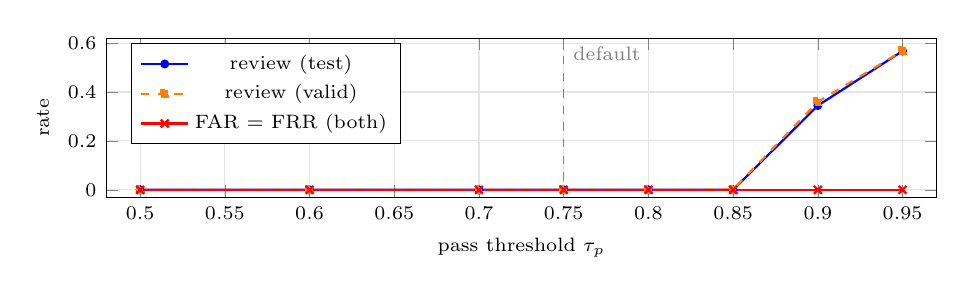
\begin{tikzpicture}
\begin{axis}[width=\columnwidth, height=36mm, xlabel={pass threshold $\tau_p$}, ylabel={rate}, ymin=-0.03, ymax=0.62, xmin=0.48, xmax=0.97,
  legend pos=north west, legend style={font=\scriptsize}, tick label style={font=\scriptsize}, label style={font=\scriptsize}, grid=major, grid style={gray!20}]
\addplot[blue, thick, mark=*, mark size=1.2pt] coordinates {(0.50,0) (0.60,0) (0.70,0) (0.75,0) (0.80,0) (0.85,0) (0.90,0.3446) (0.95,0.5678)};
\addplot[orange, thick, dashed, mark=square*, mark size=1.2pt] coordinates {(0.50,0) (0.60,0) (0.70,0) (0.75,0) (0.80,0) (0.85,0.0014) (0.90,0.3596) (0.95,0.5688)};
\addplot[red, thick, mark=x] coordinates {(0.50,0) (0.60,0) (0.70,0) (0.75,0) (0.80,0) (0.85,0) (0.90,0) (0.95,0)};
\draw[gray, dashed] (axis cs:0.75,-0.03) -- (axis cs:0.75,0.62) node[pos=0.9, right, font=\scriptsize] {default};
\legend{review (test), review (valid), FAR = FRR (both)}
\end{axis}
\end{tikzpicture}
\caption{Gate sweep with the FP16 engine ($\tau_d{=}0.45$; other $\tau_d$ values give identical curves).}
\label{fig:sweep}
\end{figure}

\textit{Images outside the dataset.} During system integration the deployed engine was also run on photographs of our own bottles, which the model had never seen in training or evaluation, and its verdicts on these were satisfactory.

\subsection{Fill-Level Estimation}
Table~\ref{tab:fill} reports both detectors on their held-out test splits at 640\,px. The meniscus detector localises the surface reliably at IoU 0.5 (AP 0.923) but loosely at strict IoU (AP@0.5:0.95 of 0.458). Because Eq.~\eqref{eq:ratio} uses only the box mid-line, this looseness affects the ratio less than the strict-IoU score suggests. FP16 conversion leaves the meniscus detector unchanged but lowers the bottle detector's AP@0.5:0.95 from 0.578 to 0.481. The deployed bottle engine is also built at 640\,px while the detector was trained at 512\,px. Building the bottle engine at its 512\,px training resolution is the planned remedy.

\begin{table}[t]
\caption{Station 2 detectors on held-out test splits (640\,px)}
\label{tab:fill}
\centering
\setlength{\tabcolsep}{3.5pt}
\begin{tabular}{llcccc}
\toprule
Model (class, $n$ boxes) & Runtime & P & R & AP$^{50}$ & AP$^{50:95}$\\
\midrule
\multirow{2}{*}{YOLOv8s (bottle, 356)} & FP32 & 0.855 & 0.880 & 0.935 & 0.578\\
 & TRT FP16 & 0.823 & 0.890 & 0.907 & 0.481\\
\multirow{2}{*}{YOLOv8n (surface, 76)} & FP32 & 0.904 & 0.867 & 0.923 & 0.458\\
 & TRT FP16 & 0.883 & 0.882 & 0.921 & 0.459\\
\bottomrule
\end{tabular}
\end{table}

To measure how meniscus localisation affects the estimate, we ran the deployed engines on the 41 surface-test images. For each, we compared the ratio from the predicted surface with the ratio from the annotated surface, using the same predicted bottle box. Table~\ref{tab:ratio} gives the results. In 31 of 35 evaluable images the ratio differs by at most 0.02, and the median difference is 1\,px. Verdicts agree in 34 of 35 images. The single disagreement is an overfilled bottle (annotated ratio 0.902) that was passed as normal (0.708).

Inspection of the large errors shows one failure mode. When the true surface sits high in the neck, the detector fires on a horizontal structure lower on the body, such as a moulded shoulder rib, a glare band, or the edge of a gripping hand. The two missed surfaces are a tinted bottle held in a hand and a nearly full bottle. All four frames with no bottle detection come from the multi-bottle rack video, which the single-bottle design does not support.

\begin{table}[t]
\caption{Fill-ratio error from meniscus localisation (41 test images, TRT FP16)}
\label{tab:ratio}
\centering
\resizebox{\columnwidth}{!}{%
\begin{tabular}{lr}
\toprule
No bottle detected (multi-bottle rack frames) & 4\\
Bottle found, no surface associated & 2\\
Evaluated & 35\\
Median $|\Delta R|$ / MAE / 90th pct. / max & 0.002 / 0.023 / 0.022 / 0.300\\
$|\Delta R|\leq0.02$ / $\leq0.05$ & 88.6\% / 91.4\%\\
Verdict agreement (under/normal/over) & 34/35 (97.1\%)\\
Gate verdicts PASS / REJECT / UNCERTAIN & 27 / 7 / 1\\
\bottomrule
\end{tabular}
}
\end{table}

\subsection{Latency}
Table~\ref{tab:lat} isolates the network from the rest of the pipeline. TensorRT FP16 reduces the three-view cap network time from 21.0\,ms (PyTorch FP32) to 7.4\,ms, a $2.8\times$ speed-up. The single-image fill detectors drop from 8.8 and 8.3\,ms to 1.3 and 1.1\,ms. ONNX Runtime on the CPU needs 510\,ms for the cap batch, which is too slow for this line. Measured end to end through the predictor, three 2048-pixel views take 20.1\,ms. About 13\,ms of that is host-side resizing and mask post-processing, which grow with batch size and are not accelerated by the engine.

\begin{table}[t]
\caption{Per-call latency (ms, median of 100) inside the production container}
\label{tab:lat}
\centering
\setlength{\tabcolsep}{3pt}
\resizebox{\columnwidth}{!}{%
\begin{tabular}{llrrr}
\toprule
Model / input & Runtime & Network & Pre+post & Wall\\
\midrule
\multirow{3}{*}{\shortstack[l]{Cap seg.,\\3 views 2048$^2$}} & PyTorch FP32 & 20.97 & 12.47 & 33.79\\
 & TRT FP16 & 7.44 & 12.35 & 20.12\\
 & ORT CPU FP32$^\ast$ & 509.89 & 16.68 & 526.43\\
\midrule
Cap seg., 3 views 640$^2$ & TRT FP16 & 7.39 & 7.56 & 15.25\\
Cap seg., 1 view 2048$^2$ & TRT FP16 & 3.90 & 4.38 & 8.59\\
\midrule
\multirow{2}{*}{Bottle det.} & PyTorch FP32 & 8.77 & 2.11 & 11.21\\
 & TRT FP16 & 1.26 & 2.07 & 3.60\\
\multirow{2}{*}{Meniscus det.} & PyTorch FP32 & 8.34 & 2.52 & 11.15\\
 & TRT FP16 & 1.13 & 2.33 & 3.76\\
\midrule
Fill engine (both det. + Eq.~\ref{eq:ratio}) & TRT FP16 & \multicolumn{3}{r}{p50 7.34 / p95 10.23}\\
Fill gate (Alg.~1) & CPU & \multicolumn{3}{r}{p50 0.028 / p99 0.059}\\
\bottomrule
\multicolumn{5}{l}{\footnotesize $^\ast$20 calls. Pre+post: Ultralytics preprocess + postprocess.}
\end{tabular}
}
\end{table}

\textit{Closed-loop stress test.} The Station~1 stress test drives the full production path inside the container for 500 cycles: TensorRT inference, extraction of mask polygons at native resolution, the gate, a synchronous SQLite (write-ahead log) transaction that stores the three raw frames with labels, and overlay rendering. It cycles through the 354 test images, grouped three per bottle. Table~\ref{tab:stress} shows the stage breakdown. The median cycle is 299\,ms, which gives 163 bottles/min unpaced. In a second run paced at 150 bottles/min for 300 cycles, the line sustained 126.7 bottles/min with a 99th-percentile cycle of 448\,ms. The JPEG decode of each 2048-pixel triplet falls outside the timed cycle, which is why the paced run fell short of 150. No database write failed in either run.

The dominant cost is not the network. Storing three 2048-pixel frames synchronously takes 176\,ms, and the inference stage (67\,ms) is mostly mask-polygon extraction at $2048^2$. Station~2's service path (both engines, gate, audit, and overlay) takes 62.8\,ms at the median and 111.5\,ms at the 99th percentile over 500 frames.

\begin{table}[t]
\caption{Station 1 closed-loop stress test, 500 unpaced cycles (ms)}
\label{tab:stress}
\centering
\begin{tabular}{lrrr}
\toprule
Stage & p50 & p95 & p99\\
\midrule
Inference (3 views, incl. mask polygons) & 67.15 & 122.17 & 124.69\\
Quality gate & 0.12 & 0.15 & 0.18\\
SQLite WAL audit (3 raw frames) & 176.48 & 251.87 & 276.67\\
Overlay rendering (3 views) & 41.59 & 43.21 & 43.91\\
\midrule
Total closed-loop cycle & 299.18 & 392.05 & 428.71\\
\bottomrule
\end{tabular}
\end{table}

\subsection{Summary Against the Stated Targets}
Table~\ref{tab:summary} compares every measured quantity with the targets set in the earlier iteration of this project, including the ones that were missed. The false-accept and false-reject limits follow from the recall ($\geq$0.97) and precision ($\geq$0.93) targets, and the 200\,ms cycle from a line rate of 300 bottles per minute.

\begin{table}[t]
\caption{All targets and outcomes (test split unless noted)}
\label{tab:summary}
\centering
\setlength{\tabcolsep}{3pt}
\resizebox{\columnwidth}{!}{%
\begin{tabular}{llrc}
\toprule
Quantity & Target & Measured & Met\\
\midrule
Cap image-level accuracy & $\geq$0.93 & 1.000 & yes\\
Cap false accept / false reject & $\leq$3\% / $\leq$7\% & 0\% / 0\% & yes\\
Cap mask mAP@0.5:0.95 (FP16) & $\geq$0.75 & 0.928 & yes\\
Cap precision / recall (FP16) & $\geq$0.93 / 0.97 & 0.998 / 1.000 & yes\\
Bottle det.\ AP@0.5 / 0.5:0.95 (FP16) & $\geq$0.88 / 0.75 & 0.907 / 0.481 & yes / no\\
Meniscus P / R (FP16) & $\geq$0.93 / 0.97 & 0.883 / 0.882 & no / no\\
Meniscus AP@0.5 / 0.5:0.95 (FP16) & $\geq$0.88 / 0.75 & 0.921 / 0.459 & yes / no\\
Fill verdict agreement & $\geq$0.93 & 0.971 (34/35) & yes\\
GPU inference, 3 views (network) & $<$100\,ms & 7.4\,ms & yes\\
GPU inference stage, p95 & $<$100\,ms & 122\,ms & no\\
Closed-loop cycle, p50 (300 bottles/min) & $\leq$200\,ms & 299\,ms & no\\
Fill service cycle, p50 / p99 & $<$100\,ms & 62.8 / 111.5\,ms & p50 only\\
CPU inference (ORT, 3 views) & $<$200\,ms & 510\,ms & no\\
\bottomrule
\end{tabular}
}
\end{table}

%=====================================================================
\section{Discussion and Limitations}
\textit{Cap station.} The distilled student is accurate, FP16-stable, and well separated by its gate thresholds. The threshold sweep also gives a monitoring rule for production: if the good-cap score distribution drifts down by more than about 0.1 (for example under new lighting or bottle types), the default $\tau_p$ will begin routing good bottles to review before any defect is passed. As the next benchmarking step (O1), we have identified a held-out test grouped by capture session, which will make results comparable across future model versions.

\textit{Distillation.} Feature alignment at C3k2, SPPF, and C2PSA lets a 22.3\,M-parameter student reproduce the 62.1\,M-parameter teacher's mAP@0.5 and surpass its mask quality at strict IoU (mask mAP@0.5:0.95 +0.015 on test, +0.023 on validation), at the cost of 0.017 box mAP@0.5:0.95. This compression is what makes the 7.4\,ms three-view engine possible. A comparison against a YOLO11m-seg trained without distillation would isolate the contribution of each distilled layer.

\textit{Fill level.} Measured against the annotated surface, the geometric rule is accurate when the meniscus is found. Its errors are detection errors rather than errors in the arithmetic. The rule assumes one upright bottle per frame and a visible meniscus inside the bottle box. Our analysis isolates meniscus error only, because the surface dataset has no bottle annotations, so bottle-box error is bounded analytically (Section~\ref{sec:sens}) rather than measured. No physical fill-volume ground truth was available.

\textit{Throughput.} Real-time capability depends on the I/O around the network more than on the network. Writing the audit record asynchronously and down-sampling the stored frames would remove most of the 299\,ms cycle. Neither is implemented in the measured system.

\textit{Reproducibility.} The datasets are public. The dataset-statistics, evaluation, and benchmark scripts and their JSON outputs accompany this paper.

%=====================================================================
\section{Conclusion}
We evaluated a two-station bottle inspector built on a distilled YOLO11m-seg cap model and a geometric fill-level rule, both deployed as TensorRT FP16 engines. Feature distillation from a YOLO11x-seg teacher yields a student that matches the teacher's mAP@0.5 of 0.995 with 2.8$\times$ fewer parameters and segments caps more precisely than the teacher (mask mAP@0.5:0.95 of 0.927 vs.\ 0.912). On the held-out split the cap station makes no product-level errors, its thresholds have a measurable margin, and FP16 does not change its accuracy. The fill station is accurate to a median of 0.002 in fill ratio wherever the meniscus is found, and its failures are traceable to specific detection modes. TensorRT reduces network latency to 7.4\,ms for three views. The closed loop is limited by synchronous image storage, not by inference.

\section*{Acknowledgment}
This work was carried out as a capstone project under the guidance of Prof.\ Nayana N Kumar, Department of CSE (Data Science), BMS College of Engineering, Bengaluru.

\begin{thebibliography}{00}
\bibitem{banus2021} N. Banús, I. Boada, P. Xiberta, P. Toldrà, and N. Bustins, ``Deep learning for the quality control of thermoforming food packages,'' \textit{Scientific Reports}, vol. 11, 2021.
\bibitem{liu2025} G. Liu, S. Zhang, L. Wang, X. Li, and G. Li, ``Research on mechanical automatic food packaging defect detection model based on improved YOLOv5 algorithm,'' \textit{PLOS ONE}, vol. 20, 2025.
\bibitem{chatchapol2024} B. Chatchapol, W. Autanan, and W. Anan, ``Liquid filling quality control system for beverage industry using image processing and CNN,'' in \textit{Proc. 24th Int. Conf. Control, Automation and Systems (ICCAS)}, 2024, pp. 1--6.
\bibitem{liakos2025} K. G. Liakos, V. Athanasiadis, E. Bozinou, and S. I. Lalas, ``Machine learning for food quality control: A systematic review,'' \textit{Foods}, vol. 14, 2025.
\bibitem{farhangi2024} O. Farhangi, E. Sheidaee, and A. Kisalaei, ``Machine vision for detecting defects in liquid bottles: An industrial application for food and packaging sector,'' \textit{Cluster Computing and Data Science}, 2024.
\bibitem{yolo11} G. Jocher and J. Qiu, ``Ultralytics YOLO11,'' 2024. [Online]. Available: https://github.com/ultralytics/ultralytics
\bibitem{yolov8} G. Jocher, A. Chaurasia, and J. Qiu, ``Ultralytics YOLOv8,'' 2023. [Online]. Available: https://github.com/ultralytics/ultralytics
\bibitem{bolya2019} D. Bolya, C. Zhou, F. Xiao, and Y. J. Lee, ``YOLACT: Real-time instance segmentation,'' in \textit{Proc. IEEE/CVF Int. Conf. Computer Vision (ICCV)}, 2019, pp. 9157--9166.
\bibitem{hinton2015} G. Hinton, O. Vinyals, and J. Dean, ``Distilling the knowledge in a neural network,'' arXiv:1503.02531, 2015.
\bibitem{romero2015} A. Romero, N. Ballas, S. E. Kahou, A. Chassang, C. Gatta, and Y. Bengio, ``FitNets: Hints for thin deep nets,'' in \textit{Proc. Int. Conf. Learning Representations (ICLR)}, 2015.
\bibitem{wang2019} T. Wang, L. Yuan, X. Zhang, and J. Feng, ``Distilling object detectors with fine-grained feature imitation,'' in \textit{Proc. IEEE/CVF Conf. Computer Vision and Pattern Recognition (CVPR)}, 2019, pp. 4933--4942.
\bibitem{capdata} ``bottle\_cap\_sdp dataset, version 7,'' Roboflow Universe, 2024, CC BY 4.0. [Online]. Available: https://universe.roboflow.com/bottlecapproject-dyaxy/bottle\_cap\_sdp
\bibitem{coco} T.-Y. Lin \textit{et al.}, ``Microsoft COCO: Common objects in context,'' in \textit{Proc. European Conf. Computer Vision (ECCV)}, 2014, pp. 740--755.
\bibitem{howard2019} A. Howard \textit{et al.}, ``Searching for MobileNetV3,'' in \textit{Proc. IEEE/CVF Int. Conf. Computer Vision (ICCV)}, 2019, pp. 1314--1324.
\bibitem{tan2021} M. Tan and Q. Le, ``EfficientNetV2: Smaller models and faster training,'' in \textit{Proc. Int. Conf. Machine Learning (ICML)}, 2021, pp. 10096--10106.
\bibitem{ma2018} N. Ma, X. Zhang, H.-T. Zheng, and J. Sun, ``ShuffleNet V2: Practical guidelines for efficient CNN architecture design,'' in \textit{Proc. European Conf. Computer Vision (ECCV)}, 2018, pp. 116--131.
\bibitem{he2016} K. He, X. Zhang, S. Ren, and J. Sun, ``Deep residual learning for image recognition,'' in \textit{Proc. IEEE Conf. Computer Vision and Pattern Recognition (CVPR)}, 2016, pp. 770--778.
\bibitem{touvron2021} H. Touvron, M. Cord, M. Douze, F. Massa, A. Sablayrolles, and H. Jégou, ``Training data-efficient image transformers \& distillation through attention,'' in \textit{Proc. Int. Conf. Machine Learning (ICML)}, 2021, pp. 10347--10357.
\bibitem{filldata1} ``fill-level dataset, version 1,'' Roboflow Universe (majid-alikhani), CC BY 4.0. [Online]. Available: https://universe.roboflow.com/majid-alikhani/fill-level
\bibitem{filldata2} ``bottle-liquid-level dataset, version 2,'' Roboflow Universe (aisut), CC BY 4.0. [Online]. Available: https://universe.roboflow.com/aisut/bottle-liquid-level
\bibitem{micikevicius2018} P. Micikevicius \textit{et al.}, ``Mixed precision training,'' in \textit{Proc. Int. Conf. Learning Representations (ICLR)}, 2018.
\bibitem{tensorrt} NVIDIA Corporation, ``NVIDIA TensorRT developer guide,'' 2025. [Online]. Available: https://docs.nvidia.com/deeplearning/tensorrt/
\bibitem{onnxruntime} ONNX Runtime developers, ``ONNX Runtime,'' 2021. [Online]. Available: https://onnxruntime.ai
\bibitem{chicco2020} D. Chicco and G. Jurman, ``The advantages of the Matthews correlation coefficient (MCC) over F1 score and accuracy in binary classification evaluation,'' \textit{BMC Genomics}, vol. 21, art. no. 6, 2020.
\end{thebibliography}

\end{document}
